\documentclass[10pt,twocolumn,letterpaper]{article}

% Barang-barang saya sendiri
\usepackage{booktabs}
% \usepackage{caption}
% \captionsetup[table]{skip=8pt}   % Hanya mempengaruhi tabel
\usepackage{stfloats}  % Tambahkan ini ke preamble
\usepackage{float}

\usepackage{cvpr}
\usepackage{times}
\usepackage{epsfig}
\usepackage{graphicx}
\usepackage{amsmath}
\usepackage{amssymb}

% Sertakan paket lain di sini, sebelum hyperref.

% Jika Anda mengomentari hyperref lalu membatalkannya, Anda harus menghapus
% egpaper.aux sebelum menjalankan latex lagi.  (Atau cukup tekan 'q' pada latex pertama
% run, let it finish, and you should be clear).
\usepackage[breaklinks=true,bookmarks=false]{hyperref}

\cvprfinalcopy % *** Uncomment this line for the final submission

\def\cvprPaperID{****} % *** Enter the CVPR Paper ID here
\def\httilde{\mbox{\tt\raisebox{-.5ex}{\symbol{126}}}}

% Pages are numbered in submission mode, and unnumbered in camera-ready
%\ifcvprfinal\pagestyle{empty}\fi
\setcounter{page}{1}
\begin{document}

%%%%%%%%% TITLE
\title{Pengantar Berbasis Data ECDO Bagian 1/2: Pemahaman Saat Ini tentang Teori Eksotermik Pemisahan Inti-Mantel dan Osilasi Dzhanibekov (ECDO) “Flip Bumi”}

\author{Junho\\
Diterbitkan Februari 2025\\
Website (Unduh makalah di sini): \href{https://sovrynn.github.io}{sovrynn.github.io}\\
Repositori Riset ECDO: \href{https://github.com/sovrynn/ecdo}{github.com/sovrynn/ecdo}\\
{\tt\small junhobtc@proton.me}
% Untuk makalah yang semua penulisnya berasal dari institusi yang sama,
% abaikan baris-baris berikut hingga penutup ``}''.
% Penulis dan alamat tambahan dapat ditambahkan dengan ``\and'',
% seperti penulis kedua.
% Untuk menghemat ruang, gunakan alamat email atau halaman rumah, jangan keduanya
% \and
% xxx
% Institusi2\\
% Baris pertama alamat institusi2\\
% {\tt\small secondauthor@i2.org}
}

\maketitle
%\thispagestyle{empty}

%%%%%%%%% ABSTRACT
\begin{abstract}
Pada bulan Mei 2024, seorang penulis daring anonim dengan nama “The Ethical Skeptic” \cite{0} membagikan sebuah teori revolusioner yang disebut Exothermic Core-Mantle Decoupling Dzhanibekov Oscillation (ECDO) \cite{1}. Teori ini menyarankan bahwa Bumi sebelumnya telah mengalami perubahan mendadak dan katastrofik pada sumbu rotasinya, yang memicu banjir besar secara global saat lautan meluap ke daratan akibat inersia rotasi. Selain itu, teori ini juga menghadirkan proses geofisika penjelas dan data yang menunjukkan kemungkinan bahwa pembalikan seperti itu bisa saja segera terjadi. Meskipun prediksi banjir katastrofik dan kiamat semacam ini bukanlah hal baru, teori ECDO memiliki daya tarik yang unik karena pendekatannya yang ilmiah, modern, multidisipliner, dan berbasis data.


This paper adalah bagian pertama dari dua bagian ringkasan singkat dari enam bulan penelitian independen \cite{2,20} tentang teori ECDO. Paper ini menyoroti tiga poin utama:

\begin{flushleft}
\begin{enumerate}
    \item 'Pembalikan Bumi' mirip ECDO telah terjadi beberapa kali dalam sejarah manusia yang baru-baru ini, seperti yang dibuktikan oleh mitos banjir dan tanda-tanda geologis banjir benua yang meluas.
    \item Arah dan besaran perkiraan pembalikan Bumi di masa lalu dapat ditentukan.
    \item Data geomagnetik dan geofisika terbaru menunjukkan bahwa pembalikan Bumi berikutnya mungkin akan segera terjadi, dan bahwa perubahan iklim mungkin disebabkan oleh perubahan di dalam Bumi yang dalam, bukan oleh manusia.
\end{enumerate}
\end{flushleft}

Selain itu, saya membahas fisika penyebab di balik “pembalikan Bumi” yang diusulkan oleh teori ECDO.

Dalam paper ini, saya tetap objektif dengan berfokus pada data yang kuat, menghindari bagian-bagian teori yang menarik tetapi spekulatif, dan menekankan bahwa ini adalah topik yang sangat mendesak untuk diteliti lebih lanjut oleh umat manusia.
\end{abstract}

%%%%%%%%% BODY TEXT
\section{Introduction}

Cerita tentang banjir besar bukanlah hal baru—faktanya, cerita ini ditemukan di setiap kebudayaan besar di seluruh dunia, mencakup semua pusat peradaban. Plotting (Gambar \ref{fig:1}) kompilasi dari 267 cerita banjir \cite{3} menunjukkan bahwa hampir semua wilayah Bumi yang dihuni memiliki cerita tentang banjir.

% \begin{figure}[h]
% \begin{figure}[b]
\begin{figure}[h]
\begin{center}
% \fbox{\rule{0pt}{2in} \rule{0.9\linewidth}{0pt}}
   \includegraphics[width=1\linewidth]{b.png}
\end{center}
   \caption{Lokasi cerita banjir di seluruh dunia \cite{3}.}
\label{fig:1}
\label{fig:onecol}
\end{figure}

Tinjauan lebih dekat terhadap cerita-cerita banjir ini menunjukkan bahwa kejadian-kejadian tersebut bukanlah banjir biasa, melainkan, bencana dahsyat yang disertai banjir yang menyapu bersih benua-benua.

\subsection{Cerita Bencana Suku Asli Amerika}

Cerita dari suku asli Amerika memuat beberapa kisah paling jelas tentang bencana besar yang menimpa Bumi. Suku Hopi, salah satu suku asli Amerika yang tinggal di timur laut Arizona, mengatakan bahwa, \textit{"..Sótuknang memanggil Rakyat Semut (Ant People) untuk membuka dunia bawah tanah mereka bagi orang-orang terpilih. Saat mereka sudah aman di bawah tanah, Sótuknang memerintahkan para kembar, Pöqánghoya dan Palöngawhoya, untuk meninggalkan pos mereka di ujung utara dan selatan poros dunia, tempat mereka ditempatkan untuk menjaga bumi tetap berputar dengan benar. \textbf{Baru saja kedua kembar itu meninggalkan pos mereka, dunia ini, tanpa ada yang mengendalikan, menjadi tidak seimbang, berputar tak terkendali, lalu berguling dua kali.} Gunung-gunung terjun ke laut dengan cipratan besar, lautan dan danau melimpah ke daratan; dan saat dunia berputar melewati ruang yang dingin dan tak bernyawa, dunia membeku menjadi es padat"} \cite{4}.

Banyak dari cerita-cerita ini secara tepat menggambarkan besarnya skala banjir, menceritakan bagaimana lautan naik hingga menenggelamkan hampir seluruh puncak gunung tertinggi. Suku Indian Skokomish, yang tinggal di negara bagian Washington, menceritakan bagaimana, \textit{"Roh Agung, marah terhadap kejahatan manusia dan hewan, memutuskan untuk membersihkan bumi dari semua kecuali hewan baik, satu orang baik, dan keluarganya. Atas arahan Roh Agung, laki-laki itu menembakkan anak panah ke awan, lalu anak panah berikutnya ke anak panah pertama, dan seterusnya, hingga membentuk tali dari anak panah dari awan ke tanah. Hewan dan manusia baik memanjat naik. Hewan buruk dan ular mencoba ikut naik, tetapi laki-laki itu memutuskan tali anak panah. \textbf{Kemudian Roh Agung menyebabkan hujan turun berhari-hari, membanjiri bumi hingga garis salju di Takhoma (Gunung Ranier).} Setelah semua manusia dan hewan jahat tenggelam, Roh Agung menghentikan hujan, air perlahan surut, dan orang serta hewan baik turun kembali"} \cite{3}. Sebagai referensi, Gunung Rainier adalah gunung berapi aktif di Washington dengan ketinggian puncak 4392,5 m di atas permukaan laut.

The flood story from the Makah Indians of Washington state specifically mentions a multi-phase flood of "very warm" waters, indicating that this was no normal flood: \textit{"Lautan naik cukup tinggi untuk memutuskan tanjung. Kemudian air surut, mencapai titik surut terendah empat hari kemudian, meninggalkan Teluk Neah kering dan tinggi. Lalu air kembali naik hingga menutupi semua kecuali puncak-puncak gunung. \textbf{Air yang naik sangat hangat.} Orang-orang dengan kano memuat barang-barang mereka dan terbawa jauh ke utara. Banyak yang meninggal ketika kano mereka tersangkut di pohon-pohon. Laut kembali normal setelah empat hari lagi, dan orang-orang mendapati diri mereka jauh di utara, di mana keturunan mereka masih tinggal"} \cite{3}.

\subsection{Cerita Bencana Alam Tiongkok}

Di sisi lain Samudra Pasifik, peradaban Tiongkok modern dikatakan dimulai dengan banjir besar. Dinasti Xia, diperkirakan ada sekitar tahun 2000 SM, didirikan oleh Yu yang Agung, yang menghentikan Banjir Besar Gun-Yu \cite{6}. Pada masanya, \textit{"... keajaiban dikatakan terjadi bahwa matahari selama sepuluh hari berturut-turut tidak terbenam, hutan-hutan terbakar, dan banyak sekali binatang-binatang menjijikkan muncul... Gelombang besar "yang mencapai langit" jatuh di tanah Tiongkok. \textbf{"Air sudah mencapai pegunungan tinggi, dan lereng-lereng sama sekali tidak terlihat"}... "Sangat merusak dalam limpahannya adalah air banjir," kata kaisar. "Dalam luasnya mereka merangkul bukit-bukit dan melampaui puncak-puncak yang tinggi, mengancam langit dengan banjirnya." Kaisar memerintahkan agar segala upaya dilakukan untuk membuka saluran keluar bagi air yang terjebak di lembah-lembah di antara pegunungan. Selama bertahun-tahun penduduk bekerja keras, mencoba membebaskan dataran dan lembah dari air banjir dengan menggali saluran dan mengeringkan ladang. Sekian lama semua usaha sia-sia. Menteri yang bertanggung jawab atas pekerjaan besar dan mendesak ini, Khwan, dihukum mati karena kegagalannya... dan hanya putranya Yu yang berhasil mengeringkan tanah itu. Prestasi ini begitu dihargai sehingga Yu menjadi kaisar Tiongkok setelah Raja Shun, penerus pertama Yahou"} \cite{5}.

Tampaknya bukan hanya Tiongkok yang dilanda banjir, tetapi juga ada kebutuhan untuk mengukur ulang arah mata angin dan pergerakan matahari serta bulan, yang mengisyaratkan bahwa rotasi Bumi mungkin telah berubah selama banjir: \textit{\textbf{"Kaisar ini mengirim para cendekiawan ke berbagai penjuru Tiongkok, dan bahkan ke Indo-Tiongkok, untuk mengetahui letak utara, barat, timur, dan selatan dengan mengamati arah terbit dan terbenamnya matahari serta gerak bintang-bintang.} Ia juga memerintahkan para ahli astronomi untuk mengetahui lamanya musim, dan membuat kalender baru... "Setelah itu Yaou [Yahou] memerintahkan He dan Ho, dengan hormat sesuai kehendak langit luas, untuk menghitung dan menggambarkan pergerakan dan penampakan matahari, bulan, bintang dan rasi zodiak; serta menyampaikan musim kepada rakyat"} \cite{5}.

Catatan bencana alam dalam sejarah Tiongkok sebenarnya sudah ada jauh sebelum Dinasti Xia, bahkan hingga periode Tiga Penguasa dan Lima Kaisar \cite{7}. Nüwa, salah satu dari Tiga Penguasa dan sosok utama Penciptaan dalam sejarah Tiongkok, menghentikan banjir saat bencana di mana Bumi berubah rotasi: \textit{"Terjadi pertengkaran antara dua dewa yang lebih kuat, dan mereka memutuskan untuk menyelesaikannya dengan bertarung. Ketika dewa air Gong Gong melihat dirinya kalah, ia membenturkan kepalanya ke Gunung Buzhou, sebuah pilar penyangga langit. \textbf{Pilar tersebut runtuh dan menyebabkan langit miring ke barat laut dan bumi bergeser ke tenggara.} Hal ini menimbulkan bencana besar, seperti kebakaran tanpa henti, banjir besar, dan kemunculan binatang buas pemakan manusia. Nüwa memotong kaki kura-kura raksasa dan menggunakannya untuk menggantikan pilar yang roboh, mengurangi situasi dan menambal langit yang rusak dengan batu dari tujuh warna berbeda, namun ia tidak mampu sepenuhnya memperbaiki langit yang miring tersebut"} \cite{8}.

\subsection{Cerita Bencana Alam Eropa, Maya, Timur Tengah, dan Asia Tenggara}

Karena ada terlalu banyak cerita bencana yang bisa dijelaskan secara terperinci dalam makalah ini, saya hanya akan menyebutkan secara singkat beberapa budaya lain yang juga memiliki kisah-kisah ini. Sastra Yunani memuat tiga kisah banjir, yaitu Deucalion, Ogyges, dan Dardanus \cite{9,10}. Dalam kisah pertama, \textit{"Setelah sembilan hari banjir, dunia hancur, dan bahtera itu berlabuh di puncak Gunung Parnassus"}, yang memiliki ketinggian puncak 2.457 meter \cite{11}. Sastra Maya meyakini ada empat Matahari yang berbeda sebelum Matahari saat ini, dan zaman Matahari keempat, Calchiuhtlicue, berakhir dengan banjir dunia pada sekitar tahun 3100 SM dan kelahiran matahari kelima yang sekarang \cite{12}. Di Timur Tengah, kronologi Alkitab memuat kisah banjir Nuh yang terkenal, dan Epos Gilgamesh, puisi Babilonia, menceritakan kisah serupa \cite{13}. Budaya Asia Tenggara juga kaya akan dongeng banjir—misalnya, orang Ot Danum di Indonesia mengatakan bahwa, \textit{"Sebuah banjir besar pernah menenggelamkan banyak orang. Beberapa orang selamat dengan melarikan diri menggunakan perahu ke satu puncak gunung yang masih tersisa di atas air. Mereka tinggal di sana selama tiga bulan hingga banjir surut"} \cite{3}. Pulau Kalimantan, tempat mereka tinggal, memiliki ketinggian puncak 4.095 meter.

\begin{figure*}[b]
\begin{center}
% \fbox{\rule{0pt}{2in} \rule{.9\linewidth}{0pt}}
\includegraphics[width=1\textwidth]{marine.jpg}
\end{center}
   \caption{Sebuah plot global fosil laut (samudra), air asin, dan cekungan/pertambangan garam \cite{15,16,86,87}.}
   \label{fig:2}
\end{figure*}

\subsection{Analisis Cerita Bencana Statistik}

Jelas, cerita-cerita ini menggambarkan banjir besar yang sering disertai oleh jenis kekuatan geofisika bencana lainnya. Analisis terhadap 117 cerita bencana (Tabel \ref{tab: 1}) menunjukkan bahwa badai api, perubahan topografi, dan perubahan rotasi Bumi sering dicatat terjadi bersamaan dengan banjir besar \cite{14}:

\begin{table}[ht]
\begin{center}
\renewcommand{\arraystretch}{1.2}  % Optional, to increase row spacing
\begin{tabular}{|l|c|c|}
\hline
\textbf{Jenis Bencana} & \textbf{Jumlah} & \textbf{Persentase Kejadian} \\
\hline\hline
Banjir besar            & 84 & 71.79 \\
Kebakaran besar/badai api & 39 & 33.33 \\
Perubahan topografi   & 29 & 24.79 \\
Gangguan bintang     & 15 & 12.82 \\
Langit runtuh           & 15 & 12.82 \\
Kegelapan berkepanjangan      & 14 & 11.97 \\
Lost lands and lakes    & 12 & 10.26 \\
Angin siklon            & 10 & 8.55  \\
Perubahan aksial/rotasi & 9 & 7.69  \\
Sungai/danau/laut mendidih & 8 & 6.84 \\
\hline
\end{tabular}
\end{center}
\caption{Kejadian Efek Bencana dalam Cerita}
\label{tab: 1}
\end{table}

Kekhususan kisah banjir yang muncul dari berbagai budaya independen di seluruh dunia, bersama dengan cerita-cerita serupa tentang peristiwa kataklismik lainnya, menunjukkan bahwa kisah-kisah banjir ini mungkin merupakan catatan langsung dari bencana yang benar-benar terjadi.

\section{Bukti Fisik untuk Banjir Lautan}

Mendukung kisah banjir tersebut, terdapat berbagai bentuk bukti fisik mengenai genangan laut yang meluas di permukaan benua Bumi. Bentuk bukti yang paling langsung antara lain garam (air asin, dataran garam, dan tambang garam) dan fosil laut (samudra), yang menutupi area luas di daratan benua Bumi. Gambar \ref{fig:2} menunjukkan plot air asin (biru), dataran dan tambang garam (coklat), serta fosil laut \cite{15,16,86,87}, yang menggambarkan sejauh mana penanda genangan laut ini.

Beberapa area yang paling menarik berisi air asin adalah dataran tinggi Himalaya di Tibet dan pegunungan Andes di Amerika Selatan, kedua area ini memiliki ketinggian rata-rata 4000 meter, yang pertama digambarkan pada Gambar \ref{fig:3}. Kisah banjir di Tibet mengatakan bahwa, \textit{"\textbf{Tibet hampir seluruhnya terendam}, sampai dewa Gya merasa iba dengan para penyintas, menarik air melalui Bengal, dan mengirim guru untuk menyejahterakan masyarakat, yang sampai saat itu masih hampir seperti monyet"} \cite{3}. Mitos Peru menggambarkan pembentukan gunung terjadi bersamaan dengan banjir yang menutupi puncak gunung: \textit{"Penggembala dan enam anaknya mengumpulkan semua makanan dan domba yang bisa mereka ambil dan membawanya ke puncak gunung sangat tinggi Ancasmarca. \textbf{Saat air banjir naik, gunung itu juga naik lebih tinggi, sehingga puncaknya tidak pernah terendam, dan kemudian gunung itu turun bersama airnya.} Enam anak tersebut mengisi kembali penduduk provinsi setelah banjir"} \cite{3}.

\begin{figure}[t]
\begin{center}
% \fbox{\rule{0pt}{2in} \rule{0.9\linewidth}{0pt}}
   \includegraphics[width=1\linewidth]{tibet.jpg}
\end{center}
   \caption{Peta topografi Himalaya yang menunjukkan air asin (biru kehijauan), garam kering (putih), dan fosil laut (merah) \cite{15,16,86,87}.}
\label{fig:3}
\label{fig:onecol}
\end{figure}

Sementara aliran pemikiran geologi uniformitarian menganggap anomali seperti garam dan fosil laut sebagai proses panjang yang terjadi selama jutaan tahun, kisah-kisah banjir umat manusia seharusnya membuat kita mempertanyakan pola pikir tersebut. Jika samudra benar-benar membanjiri benua, maka air asin dan fosil laut, yang mudah ditemukan di hamparan luas daratan berketinggian tinggi, adalah persis seperti yang kita harapkan untuk ditemukan.

\begin{figure*}[t]
\begin{center}
\includegraphics[width=0.85\textwidth]{khafre.jpg}
\end{center}
   \caption{Diagram yang menunjukkan erosi karst berpola dan berbeda-beda akibat kenaikan permukaan laut sementara yang berlangsung lama \cite{27}.}
\label{fig:4}
\end{figure*}

\subsection{Anomali Fisik Tambahan}
There are numerous other forms of anomalies that uniformitarian science fails to explain. Mammoth beku-sempurna yang terawetkan dengan baik terkubur dalam lumpur dengan daging yang masih dapat dimakan setelah ribuan tahun \cite{17,18,19}, lembaran besar sedimen bertumpuk yang terdeposit secara horizontal di Amerika Utara yang membentang seluas 2,4 juta km$^2$ \cite{21}, lanskap riak arus besar \cite{22}, dan batu-batu aneh yang berasal dari ratusan kilometer jauhnya tergeletak di puncak gunung \cite{23,26} hanyalah beberapa fenomena yang oleh geologi uniformitarian modern dijelaskan secara dangkal dengan penjelasan umum seperti "proses yang lama dan berlarut-larut." Anomali semacam ini paling baik dijelaskan melalui kekuatan geofisik katastropik, dan akan dibahas pada bagian kedua makalah ini.

Selain itu, pergeseran dan pembalikan kutub geomagnetik secara luas diterima sebagai fenomena berulang di Bumi, berdasarkan data paleomagnetik \cite{35,40,41}. Namun, sains modern gagal menjelaskan secara pasti mengapa dan bagaimana pembalikan kutub ini terjadi.

\section{ECDO dan Piramida Giza}

Piramida Khafre dan Khufu di Giza adalah salah satu titik fokus utama dalam tesis ECDO Ethical Skeptic \cite{27}, karena tidak hanya memberikan bukti tentang banjir samudra sementara yang berlangsung lama tetapi juga menunjukkan arah potensial perubahan ECDO Bumi, menyiratkan bahwa nenek moyang kita mampu mengukur bencana Bumi dan memiliki keterampilan rekayasa untuk menanamkan pengetahuan ini dalam struktur batu besar yang sangat direkayasa. Kedua piramida ini, yang konon dibangun sekitar 2500 SM sebagai makam bagi firaun Khufu dan Khafre, keduanya terletak di Mesir utara pada sekitar (30 N, 31 E). Piramida ini memiliki dasar lebih dari 200 meter, dan tingginya sekitar 140 meter. Piramida Khufu dibangun dengan menggunakan sekitar 2,3 juta blok batu kapur, masing-masing dengan berat rata-rata lebih dari dua ton \cite{24, 25}.

Terdapat banyak ketidakpastian seputar asal usul piramida ini, yang dibahas Ethical Skeptic dalam tesisnya. Ia menunjukkan banyak ketidakkonsistenan dalam narasi konvensional seputar piramida, menunjukkan, paling tidak, tingkat kebingungan signifikan terkait umur dan sejarah piramida:

\begin{flushleft}
\begin{itemize}
    \item Penanggalan karbon pada mortar kuno di sekitar dan alat perampok makam menunjukkan bahwa piramida kemungkinan dibangun jauh lebih awal daripada yang diyakini secara konvensional.
    \item Tanda-tanda tambang yang disebut-sebut ditemukan di ruang internal piramida Khufu mencurigakan dari segi penempatannya, material, tingkat pelestarian, penggunaan hieroglif Mesir, dan waktu/sifat penemuan, sehingga menunjukkan kemungkinan pemalsuan. Mereka juga berbeda dari tanda oker kuno asli lain yang ditemukan di bagian piramida yang lain.
    \item Erosi karst diferensial pada Sphinx terdekat tidak sesuai dengan narasi konvensional mengenai konstruksinya.
\end{itemize}
\end{flushleft}

\begin{figure*}[b]
\begin{center}
\includegraphics[width=0.85\textwidth]{shafts.jpg}
\end{center}
   \caption{Poros dan ruang interior Piramida Khufu, yang menurut Ethical Skeptic merupakan observatorium pemantauan geofisika tripartit untuk peristiwa ECDO \cite{28}.}
\label{fig:5}
\end{figure*}

Salah satu area utama yang diselidiki dalam tesis Ethical Skeptic adalah erosi diferensial berpola di bagian luar Piramida Khafre, yang digambarkan pada Gambar \ref{fig:4}. Ujung piramida mempertahankan lapisan luar batu kapur Tura yang lembut, yang dulunya menutupi seluruh piramida. Ujung lapisan batu kapur ini hanya mengalami pelapukan ringan, tetapi terletak tepat di atas lapisan tipis yang telah mengalami erosi karst berat, memperlihatkan batu kapur Mokkatam Mohs 7 yang lebih keras yang digunakan untuk blok struktural bagian dalam piramida. Di bawahnya, tubuh piramida mempertahankan lapisan batu kapur Tura Mohs 4 yang telah mengalami erosi karst berat. Intinya di sini adalah bahwa batu kapur Tura yang lebih lunak pada lapisan luar piramida, yang terdiri dari CaCO$_3$, dapat larut dalam air dalam kondisi tertentu. Ethical Skeptic mengutip lapisan erosi karst berat yang selektif berhenti pada batu kapur Mokkatam yang keras, erosi pola gelombang di sudut-sudut ujung, dan perbedaan antara pelapukan ringan pada ujung yang tinggi dengan erosi karst berat pada bagian bawah badan piramida, sebagai bukti jelas adanya kenaikan tingkat permukaan laut yang berlangsung lama dan kemudian surut dengan cepat \cite{27}.

\begin{figure*}[b]
\begin{center}
% \fbox{\rule{0pt}{2in} \rule{.9\linewidth}{0pt}}
\includegraphics[width=1\textwidth]{drawing.jpg}
\end{center}
   \caption{Ilustrasi rotasi ECDO yang diusulkan, bergerak 104 derajat ke utara sepanjang bujur timur ke-31, dengan tanda silang menggambarkan pivot timur dan barat serta penanda merah menunjukkan lokasi Piramida Khufu.}
\label{fig:6}
\end{figure*}

Ethical Skeptic juga sangat menyoroti desain internal dan kondisi Piramida Khufu (Gambar \ref{fig:5}) dalam penelitiannya \cite{28}. Piramida Khufu memiliki beberapa ruang (Ruang Raja, Ratu, dan Bawah Tanah), berbagai koridor dan poros, serta dua pasang apa yang disebut "poros udara", dengan masing-masing pasangan memancar keluar dari Ruang Raja dan Ruang Ratu \cite{29,30}. Dalam makalah ini, kami hanya akan membahas bagian terpenting dari penyelidikan Ethical Skeptic—yaitu orientasi dan desain dua pasang "poros udara", karena ini memuat informasi penting tentang arah perubahan ECDO Bumi.
The key here is understanding that the shafts were built to point very precisely towards certain directions. First off, both pairs of shafts currently point directly north and south. Additionally, they were each built with an inner angle of 104 degrees.

Kunci di sini adalah memahami bahwa lorong-lorong tersebut dibangun untuk menunjuk sangat tepat ke arah-arah tertentu. Pertama, kedua pasang lorong tersebut saat ini menunjuk langsung ke utara dan selatan. Selain itu, masing-masing dibangun dengan sudut dalam 104 derajat.

The most telling clue, however, is a celestial star map carved on the interior of one of the Queen's shafts. This star map is centered around a celestial north pole orientation from approximately 9600 to 9200 BCE, based on the precession of the equinoxes \cite{28}. This suggests a deliberate orientation of the shafts, and that at the time of construction, one pair of shafts from the King and Queen's Chamber's pointed towards the celestial north pole. This begs the question - what do the other ends of the shafts point towards, and why were they both built with an angle of 104 degrees? Ethical Skeptic proposes that these were built to align with the celestial north pole following a 104-degree ECDO flip.

Namun, petunjuk paling jelas adalah sebuah peta bintang langit yang dipahat di bagian dalam salah satu lorong Ratu. Peta bintang ini berpusat pada orientasi kutub utara langit dari sekitar tahun 9600 hingga 9200 SM, berdasarkan presesi ekuinoks \cite{28}. Ini menunjukkan adanya orientasi sengaja dari lorong-lorong tersebut, dan bahwa pada saat dibangun, sepasang lorong dari Kamar Raja dan Ratu mengarah ke kutub utara langit. Ini menimbulkan pertanyaan – ke mana ujung lain dari lorong-lorong tersebut menunjuk, dan mengapa keduanya dibangun dengan sudut 104 derajat? Ethical Skeptic mengusulkan bahwa lorong-lorong tersebut dibuat untuk sejajar dengan kutub utara langit setelah terjadi pembalikan ECDO sebesar 104 derajat.

\section{Bukti untuk Rotasi 104 Derajat Sepanjang Meridian ke-31}

Ethical Skeptic dengan demikian mengusulkan bahwa Bumi mengalami pembalikan berulang 104 derajat sepanjang meridian ke-31, di mana Piramida Khufu dan lorong gandanya berada. Gambar \ref{fig:6} menunjukkan rotasi yang diprediksi, bersama dengan "poros" timur (Indonesia, 121 derajat BT) dan barat (Amerika Selatan, 59 derajat BB), dua lokasi yang tidak akan bergeser posisinya setelah terjadi pembalikan sepanjang meridian ke-31. Setelah Bumi berotasi ke keadaan baru ini, diperkirakan akan tetap berada di sana untuk sementara waktu (beberapa dekade hingga abad) sebelum kembali ke keadaan "normal" saat ini \cite{150}.

Salah satu kisah bencana yang sangat relevan diceritakan oleh Herodotus, sejarawan paling terkenal di Yunani kuno, yang hidup pada abad kelima SM \cite{31}. Dalam bukunya "An Account of Egypt," Herodotus menceritakan bagaimana para imam Mesir berkata kepadanya, \textit{"...dari raja pertama hingga imam Hephaistos yang terakhir memerintah, ada tiga ratus empat puluh satu generasi manusia... tetapi tiga ratus generasi manusia sama dengan sepuluh ribu tahun, karena seratus tahun adalah tiga generasi manusia... Maka dalam kurun sebelas ribu tiga ratus empat puluh tahun mereka berkata bahwa tidak ada dewa yang muncul dalam wujud manusia; bahkan sebelum atau sesudah masa itu di antara raja-raja lain yang muncul di Mesir, mereka tidak melaporkan bahwa hal seperti itu pernah terjadi. \textbf{Pada masa itu mereka berkata bahwa matahari telah berpindah empat kali dari tempat terbit biasanya, dan di mana sekarang ia terbenam, ia dua kali telah terbit dari sana, dan di tempat di mana sekarang ia terbit ia dua kali telah terbenam;} dan selama itu tidak ada yang berubah di Mesir dari keadaan biasanya, baik yang berasal dari bumi maupun dari sungai, atau yang terkait penyakit atau kematian"} \cite{32}. Imam Hephaistos dapat diperkirakan berasal dari awal abad ke-7 SM, karena ia sezaman dengan Sennacherib, raja Kekaisaran Neo-Asiria, sebagaimana dinyatakan sendiri oleh Herodotus \cite{32,33,34}.

Cerita ini penting karena memberi tahu kita bahwa ketika Matahari berpindah di Mesir, ia \textit{secara khusus menukar tempat terbit dan terbenamnya}. Ini hanya dapat terjadi jika Mesir berputar 180 derajat dan tetap berada pada lintang yang serupa. Ketika kita mempertimbangkan desain piramida dan data yang dibahas pada subbagian berikutnya, kita dapat menyimpulkan bahwa Mesir mungkin terletak di meridian tempat Bumi berotasi ke posisinya yang baru (meridian timur ke-31).

Mesir adalah satu-satunya \textit{lokasi} di Bumi dengan cerita yang menyebutkan bahwa Matahari secara khusus bertukar tempat terbit dan terbenamnya. Satu-satunya cerita lain di dunia yang menceritakan arah spesifik rotasi Bumi adalah cerita Nüwa dari Tiongkok, yang menyatakan bahwa, \textit{"Pilar itu runtuh dan menyebabkan langit miring ke barat laut dan bumi bergeser ke tenggara"} \cite{8}. Arah rotasi ini juga sesuai dengan arah rotasi yang diusulkan.

\subsection{Bukti Fisik untuk Rotasi 104 Derajat Sepanjang Meridian ke-31}

Bukti fisik yang mendukung arah rotasi ini meliputi data paleomagnetik, tektonik, gurun, keanekaragaman hayati, paleokurenn, dan data glasial erratic.

Sebuah studi tentang data paleomagnetik yang merekam jalur kutub geomagnetik dari peristiwa Basin Island dan Laschamp \cite{35}, yang digambarkan dalam Gambar \ref{fig:7}, menunjukkan kutub berotasi kira-kira di sekitar poros ECDO timur pada (0 LU, 121 BT). Data ini tercatat dalam jenis mineral magnetik tertentu pada batuan yang terbentuk selama peristiwa pergeseran kutub, sehingga menyimpan informasi tentang arah dan intensitas medan magnet Bumi pada saat itu.
\begin{figure}[t]
\begin{center}
% \fbox{\rule{0pt}{2in} \rule{0.9\linewidth}{0pt}}
   \includegraphics[width=0.95\linewidth]{laj.jpg}
\end{center}
   \caption{Lintasan kutub geomagnetik virtual untuk (a) peristiwa penyimpangan Cekungan Islandia dan (b) peristiwa penyimpangan Laschamp \cite{35}.}
\label{fig:7}
\label{fig:onecol}
\end{figure}

\begin{figure}[t]
\begin{center}
% \fbox{\rule{0pt}{2in} \rule{0.9\linewidth}{0pt}}
   \includegraphics[width=1\linewidth]{meinesz3.jpg}
\end{center}
   \caption{Ilustrasi pola geser pada kerak Bumi \cite{36}.}
\label{fig:8}
\label{fig:onecol}
\end{figure}
\begin{figure*}[t]
\begin{center}
% \fbox{\rule{0pt}{2in} \rule{.9\linewidth}{0pt}}
\includegraphics[width=0.95\textwidth]{biodiversity.jpg}
\end{center}
   \caption{Gambaran tentang gurun utama di dunia dan hotspot keanekaragaman hayati yang bergantian \cite{28}.}
\label{fig:9}
\end{figure*}

Sebuah studi tentang bidang geser (sesar) di kerak Bumi (Gambar \ref{fig:8}), di mana kerak Bumi telah retak atau mengalami deformasi, juga mengikuti pola yang sama. Felix Meinesz, seorang geofisikawan Belanda, menjelaskan dalam makalahnya \cite{36} bahwa alasan paling mungkin untuk pola ini adalah pergeseran sumbu rotasi Bumi.

Lokasi gurun utama di dunia dan hotspot keanekaragaman hayati juga sejajar dengan pola ini. Gurun-gurun tersebut berada di lokasi yang diperkirakan akan dibanjiri sedimen dalam jumlah besar, sementara hotspot keanekaragaman hayati berada di area yang tidak terlalu terdampak oleh perpindahan samudra \cite{28}. Keselarasan ini digambarkan pada Gambar \ref{fig:9}.

Keselarasan seperti ini terhadap jalur rotasi ECDO yang diprediksi juga terdapat pada paleokorenten sedimen yang terawetkan di lapisan batupasir di Amerika Serikat bagian barat \cite{21}, dan "glacial erratics", yaitu batuan yang\begin{figure*}[t]
\begin{center}
% \fbox{\rule{0pt}{2in} \rule{.9\linewidth}{0pt}}
\includegraphics[width=0.95\textwidth]{biodiversity.jpg}
\end{center}
   \caption{Gambaran tentang gurun utama dunia dan hotspot keanekaragaman hayati yang bergantian \cite{28}.}
\label{fig:9}
\end{figure*}

Sebuah studi tentang bidang geser (sesar) di kerak Bumi (Gambar \ref{fig:8}), di mana kerak Bumi telah retak atau mengalami deformasi, juga mengikuti pola yang sama. Felix Meinesz, seorang geofisikawan Belanda, menjelaskan dalam makalahnya \cite{36} bahwa alasan paling mungkin untuk pola ini adalah pergeseran sumbu rotasi Bumi.

Lokasi gurun utama dunia dan hotspot keanekaragaman hayati juga selaras dengan pola ini. Gurun-gurun tersebut berada di lokasi yang diperkirakan akan mengalami pembanjiran sedimen secara besar-besaran, sedangkan hotspot keanekaragaman hayati berada di wilayah yang tidak terlalu terkena dampak perpindahan samudra \cite{28}. Keselarasan ini digambarkan pada Gambar \ref{fig:9}.

Penyesuaian seperti ini terhadap jalur rotasi ECDO yang diprediksi juga ditemukan pada paleokorenten sedimen yang tersimpan di lapisan batu pasir di Amerika Serikat bagian barat \cite{21}, dan glacial erratics, yaitu batuan yang telah terangkat, diduga oleh gletser, dan diendapkan di tempat lain di atas batuan dasar yang jenis batunya berbeda dengan batuan erratic tersebut. Di Inggris Raya, batuan erratic ini mengikuti jalur aliran yang sesuai dengan rotasi ECDO \cite{67,68}.

\section{Fisika Penyebab Dibalik Pembalikan ECDO}

\begin{figure*}
\begin{center}
% \fbox{\rule{0pt}{2in} \rule{1\linewidth}{0pt}}

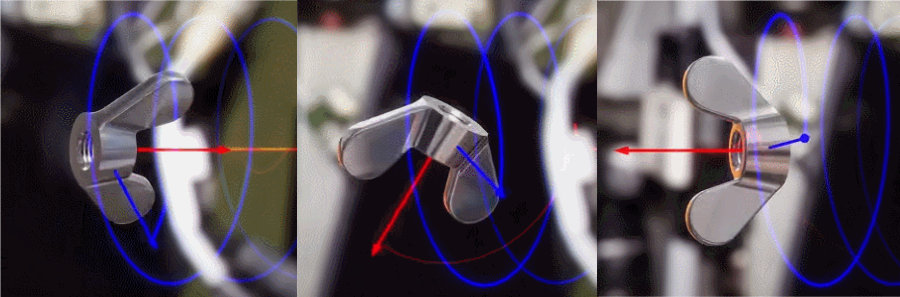
\includegraphics[width=0.9\textwidth]{dzhani.jpg}
\end{center}
   \caption{Sebuah gambaran tentang efek Dzhanibekov \cite{28}.}
\label{fig:10}
\end{figure*}

Prinsip di balik perubahan cepat pada sumbu rotasi Bumi terletak pada fisika benda berputar. Contoh kanonik dari hal ini adalah efek Dzhanibekov, yang ditemukan oleh kosmonot Rusia Vladimir Dzhanibekov \cite{37}, dan digambarkan pada Gambar \ref{fig:10}. Sebuah objek yang tidak berputar dengan sempurna pada salah satu dari tiga sumbu inersia utamanya tidak akan mempertahankan sumbu rotasi yang tetap. Jika objek tersebut berputar dekat dengan sumbu utama keduanya, ia akan mengalami perubahan rotasi yang tampak tiba-tiba. Meskipun ini tidak persis seperti yang diyakini terjadi selama pembalikan cepat Bumi, intinya adalah bahwa tanpa adanya gaya eksternal, hanya fisika rotasi yang dapat menjelaskan perubahan sumbu rotasi Bumi yang terjadi secara cepat.

Secara tepat, Bumi hampir pasti tidak mengalami efek Dzhanibekov yang sederhana dan seragam. Jika demikian, kita akan dapat mendeteksi pergeseran gradual pada sumbu rotasi Bumi dari waktu ke waktu. Sebaliknya, diyakini bahwa Bumi mengalami gangguan fisik yang periodik dan tiba-tiba, yang menyebabkan terlepasnya “rotasi luar” (kerak/mantel) dan “badan rotasi dalam” (inti). Tanpa masukan eksternal, hukum kekekalan momentum sudut menyatakan bahwa Bumi tidak bisa tiba-tiba mengubah sumbu rotasinya, sehingga pelepasan antara badan rotasi luar dan dalam adalah salah satu dari sedikit hal, selain dampak eksternal pada Bumi, yang dapat menyebabkan perubahan sumbu secara tiba-tiba dan mendadak.

Proses khusus yang mendorong gangguan internal di Bumi diyakini merupakan perubahan keadaan pada struktur besi yang membentuk inti Bumi (Gambar \ref{fig:11}). Inti dalam terdiri dari Besi (Fe) dengan struktur hexagonal close-packed \cite{141}. Ketika hcp-Fe ini berubah menjadi keadaan cair logam, energi kinetik dilepaskan dan bergerak ke inti luar. Perubahan fasa ini menurunkan permeabilitas magnetik inti, melemahkan medan geomagnetik, dan melepaskan panas, yang menciptakan struktur LLVP (large low-velocity shear province) (Gambar \ref{fig:12}) \cite{38} di mantel, serta memanaskan permukaan Bumi melalui laut abyssal. Kedua kecenderungan ini telah didokumentasikan dengan baik dalam beberapa abad terakhir dan akan dibahas lebih lanjut dalam makalah ini.

\begin{figure*}[t]
\begin{center}
% \fbox{\rule{0pt}{2in} \rule{.9\linewidth}{0pt}}
\includegraphics[width=1\textwidth]{layers.jpg}
\end{center}
   \caption{Ilustrasi proses di dalam Bumi yang menyebabkan pembalikan ECDO \cite{129}.}
\label{fig:11}
\end{figure*}
\begin{figure}[t]
\begin{center}
% \fbox{\rule{0pt}{2in} \rule{0.9\linewidth}{0pt}}
   \includegraphics[width=1\linewidth]{llvp.jpg}
\end{center}
   \caption{Visual detail dari LLVP di bawah Afrika Selatan \cite{28}.}
\label{fig:12}
\label{fig:onecol}
\end{figure}

Proses yang sama di dalam Bumi, yang terjadi secara terbalik, juga diyakini mendorong perpindahan kembali ke keadaan rotasi Bumi saat ini relatif cepat setelah pembalikan terjadi.

\section{Bukti Akan Terjadinya Pembalikan Bumi}

Ada alasan kuat untuk percaya bahwa kita berada di ambang pembalikan Bumi berikutnya. Sebuah bencana belum terjadi selama beberapa milenium, yang kira-kira sesuai dengan frekuensi terjadinya peristiwa ini berdasarkan catatan sejarah dan data. Data terkuat yang mendukung pembalikan yang akan datang berasal dari data geomagnetik terbaru, yang menunjukkan bahwa medan geomagnetik Bumi telah melemah selama kurang lebih dua ribu tahun. Pelemahan ini telah meningkat dan mencapai tingkat yang mengkhawatirkan dalam beberapa dekade terakhir.

Terlihat pada Gambar \ref{fig:14} adalah medan geomagnetik Bumi pada tahun 1590 dan 2025 \cite{125,126}. Seperti yang diperlihatkan pada gambar, medan tersebut telah melemah secara signifikan.
Another metric untuk melemahnya medan geomagnetik adalah posisi kutub utara geomagnetik (Gambar \ref{fig:13}). Kutub utara geomagnetik secara historis terletak di Arktik Kanada. Namun, ia telah bergerak perlahan selama beberapa abad terakhir, dan percepatannya meningkat secara signifikan beberapa dekade yang lalu. Sekarang, ia bergerak cepat menuju Rusia dengan kecepatan 55 kilometer per tahun \cite{124}.

\begin{figure*}[t]
\begin{center}
% \fbox{\rule{0pt}{2in} \rule{.9\linewidth}{0pt}}
\includegraphics[width=0.9\textwidth]{saa.jpg}
\end{center}
   \caption{Ilustrasi pelemahan medan geomagnetik dari tahun 1590 hingga 2025. Dihitung menggunakan model gufm1 dan IGRF-14 \cite{125,126}.}
\label{fig:14}
\end{figure*}

\begin{figure}[t]
\begin{center}
% \fbox{\rule{0pt}{2in} \rule{1\linewidth}{0pt}}
   \includegraphics[width=1\linewidth]{npw.jpg}
\end{center}
   \caption{Posisi kutub utara geomagnetik dari tahun 1590 hingga 2025, ditampilkan dalam interval 5 tahun \cite{142}.}
\label{fig:13}
\label{fig:onecol}
\end{figure}

\begin{figure}[t]
\begin{center}
% \fbox{\rule{0pt}{2in} \rule{1\linewidth}{0pt}}
   \includegraphics[width=1\linewidth]{ocean-highlight.jpg}
\end{center}
   \caption{Laju pemanasan laut dalam ($>$2000 m kedalaman) dari tahun 1991 hingga 2010, dilingkari merah \cite{132}.}
\label{fig:15}
\label{fig:onecol}
\end{figure}

Medan magnet Bumi diyakini dihasilkan oleh dinamo bagian dalam - kolom-kolom melingkar arus magma yang bergerak di inti luar Bumi akibat rotasinya \cite{123}. Pelemahan medan geomagnetik merupakan gejala gangguan yang terjadi jauh di dalam Bumi. Menurut teori ECDO, gangguan ini mengeluarkan panas dan akhirnya menyebabkan pelepasan antara mantel dan inti, yang menyebabkan terjadinya flip Bumi \cite{1}.

Terdapat banyak data yang mendukung keberadaan proses eksotermik di dalam Bumi. Pemanasan Bumi didokumentasikan melalui naiknya suhu permukaan benua dan lautan \cite{127,128}, meningkatnya tingkat CO2 atmosfer yang bergerak sejalan dengan plume panas Bumi \cite{129,130}, serta penurunan luas es laut global \cite{131}. Data ini menunjukkan bahwa kenaikan CO2 dan suhu bukanlah penyebab "perubahan iklim buatan manusia", melainkan efek hilir dari inti yang bersifat eksotermik \cite{129}.

Yang paling signifikan, studi mengenai laju pemanasan di laut dalam (kedalaman $>$2000 meter) menunjukkan bahwa tidak hanya lautan dalam mengalami pemanasan, laju pemanasan paling kuat ditemukan di lapisan abyssal (4000 - 6000 m). Pemanasan laut dalam ini memiliki titik pusat di bawah 4000 meter \cite{132,129}, yang tidak mungkin terjadi jika lautan hanya dipanaskan dari atas oleh atmosfer. Data seperti ini memberikan dukungan kuat pada pendapat bahwa perubahan iklim dan geomagnetik akhir-akhir ini didorong oleh proses-proses yang terjadi jauh di dalam Bumi. Gambar \ref{fig:15} menggambarkan laju pemanasan laut dalam global dari tahun 1991 hingga 2010 \cite{132}.

\section{Pemodelan Flip Bumi yang Akan Datang}
\begin{figure}[b]
\begin{center}
% \fbox{\rule{0pt}{2in} \rule{1\linewidth}{0pt}}
   \includegraphics[width=1\linewidth]{saa-crop.jpeg}
\end{center}
   \caption{Perhitungan tipping point berdasarkan Anomali Atlantik Selatan menunjukkan tanggal 13 Maret 2059 \cite{125,126}.}
\label{fig:16}
\label{fig:onecol}
\end{figure}

Memprediksi waktu terjadinya pembalikan Bumi berikutnya adalah tugas yang kompleks. Saat ini, model terbaik yang kita miliki untuk hal ini terletak pada medan geomagnetik Bumi - Anomali Atlantik Selatan (SAA). Wilayah ini di atas Samudra Atlantik Selatan memiliki kekuatan medan geomagnetik terlemah dan didefinisikan sebagai area dengan kekuatan medan di bawah 32.000 nanotesla \cite{135}, yang merupakan nilai medan terlemah pada tahun 1590. Luas permukaan Anomali Atlantik Selatan meningkat dari 1\% permukaan Bumi pada tahun 1590 menjadi 21\% pada tahun 2025 \cite{136}.

Untuk mendapatkan perkiraan kapan Bumi dapat mengalami pembalikan, saya menyesuaikan data luas permukaan SAA dengan persamaan tipping point power-law, yang memodelkan sistem kompleks yang mendekati transisi kritis, di mana sistem mengalami perubahan drastis dan tiba-tiba. Perhitungan saya menghasilkan prediksi tanggal tipping point pada 13 Maret 2059 (Gambar \ref{fig:16}). Prediksi ini akan menjadi semakin akurat semakin dekat kita dengan masa transisi \cite{136}.

Metrik lain seperti pergeseran sumbu rotasi, anomali cuaca, serta data seismik dan vulkanik juga dapat membantu kita untuk mendapatkan prediksi yang lebih baik tentang kapan kemungkinan terjadinya pembalikan Bumi berikutnya.

\section{Garis Waktu Historis ECDO}

Meskipun menetapkan garis waktu yang pasti untuk kejadian ECDO di masa lalu sulit, tampaknya setidaknya ada 2 kejadian ECDO selama Holosen. Perhatikan kisah yang diceritakan oleh Herodotus dari para pendeta Mesir bahwa, \textit{"dari raja pertama hingga pendeta Hephaistos yang terakhir memerintah, telah ada tiga ratus empat puluh satu generasi manusia... Dalam waktu ini mereka mengatakan bahwa matahari telah berpindah empat kali dari tempat terbit biasanya, dan di tempat yang sekarang ia terbenam, dari sana dua kali ia telah terbit, dan di tempat dari mana ia sekarang terbit dua kali ia telah terbenam"} \cite{32}. Plato, yang hidup pada abad kelima SM \cite{111}, menyatakan bahwa setelah banjir yang menenggelamkan Atlantis dalam sehari semalam 9.000 tahun sebelumnya, \textit{"sejak saat itu telah terjadi banyak banjir, dan orang-orang yang selamat di pegunungan tidak mengetahui seni menulis, dan selama banyak generasi sepenuhnya berfokus pada upaya bertahan hidup"} \cite{112}, yang menunjukkan bahwa kemungkinan telah terjadi lebih dari dua kali pembalikan sejak akhir Younger Dryas sekitar tahun 9700 SM. Bukti fisik yang telah dijelaskan dalam makalah ini dan dalam penelitian saya \cite{2} memberikan banyak bukti untuk mendukung kisah Plato.
The most recent candidate date for an ECDO flip is during the period of 2300 to 1600 SM, to which many cataclysmic flood accounts (Gun-Yu \cite{113,114,115}, Ogyges \cite{116,117}, Peru \cite{118,119}, Exodus \cite{120}), kehancuran dan pengabaian peradaban (Mohenjo-Daro \cite{121}, Minoan Crete\cite{100,101}) dan anomali fisik (peristiwa bond \cite{122}, peristiwa 4.2 kilotahun \cite{90}) telah diberi tanggal. Tidak ada konvergensi bukti yang cukup mutakhir setelah periode ini yang menunjukkan suatu kejadian bencana besar.

\section{Kesimpulan}

Operasi NANOOK adalah upaya pengintaian Perang Dingin yang dilakukan Amerika Serikat untuk memetakan Arktik dan Pesisir Utara Soviet setelah Perang Dunia II \cite{137}. Selama investigasi mereka, ditemukan bahwa kutub magnet sekitar 125 hingga 200 mil di utara dari posisi yang seharusnya berdasarkan temuan ekspedisi sebelumnya. Terkait hal tersebut, \textit{"Di antara para ilmuwan pemerintah, muncul pertanyaan mengenai apa yang akan terjadi ketika kutub magnet dan geografis berimpit. Untuk menjawab hal ini, di bawah pengawasan proyek Dr. Paul A. Siple, Rand Corporation dikontrak untuk melakukan studi laboratorium menggunakan model bumi yang terdiri dari bola-bola konsentris – bola dalam mewakili inti besi cair bermuatan elektromagnetik bumi yang porosnya mendefinisikan kutub “magnet”; dan bola luar mewakili kerak bumi yang berputar mengelilingi sumbu kutub “geografis”. Melalui percobaan berulang-ulang, ditentukan bahwa ketika kutub “magnet” mendekati kutub “geografis”, kutub “magnet” pada satu titik akan mempercepat laju konvergensinya seolah tertarik ke kutub “geografis” oleh gaya sentripetal dan melompat untuk berimpit; namun alih-alih berimpit, kutub “magnet” akan dengan cepat “membalik” mengelilingi kutub “geografis”, lalu lepas menuju ekuator seolah karena gaya sentrifugal, dan berakhir di posisi di mana kedua sumbu membentuk divergensi sekitar 89 derajat. Setelah “pembalikan” kutub terjadi, sumbu-sumbu tersebut akan kembali sedikit demi sedikit berkumpul selama waktu yang lama"} \cite{138,139}.

Selanjutnya, \textit{"Pada salah satu pertemuan ilmiah yang dihadiri Mayor White di Pentagon pada awal 1948, para ilmuwan mendiskusikan apakah perlu memberi peringatan kepada publik tentang fenomena pembalikan kutub yang akan datang. Tidak ada ilmuwan yang setuju untuk menyembunyikan informasi dari publik; namun, di sisi lain, mereka juga tidak sepakat mengenai bagaimana cara mengumumkannya. Pengetahuan tentang fenomena ini, menurut beberapa orang, dapat menghancurkan moral masyarakat. Ketakutan mereka ternyata tidak berdasar ketika, pada awal 1950-an, informasi tentang fenomena pembalikan ini dipublikasikan baik di kolom koran maupun di sebuah artikel majalah, tetapi secara mengejutkan tidak mendapat tanggapan dari publik yang tampaknya terdiam, berpikiran sempit, atau tak percaya"} \cite{138,139}.

Mengapa kita tidak memperhatikan hal ini? Ada banyak alasan untuk percaya bahwa Bumi pernah mengalami pembalikan sebelumnya. Makalah ini, bersama bagian keduanya, memberikan ringkasan padat tentang konvergensi besar bukti dari banyak bidang yang menunjukkan hal ini, seperti kisah banjir dari seluruh dunia, garam dan fosil laut yang menutupi benua, tempat perlindungan bawah tanah kuno, sisa-sisa hewan, dan lanskap geologi yang penuh bencana. Manusia konon telah berusia ratusan ribu tahun, namun sejarah modern hanya tercatat beberapa ribu tahun. Mungkinkah kadang-kadang, Bumi berbalik, benua-benua bersih dari kehidupan, dan kita dipaksa memulai kembali dari awal — Zaman Batu — sehingga catatan kita tentang sejarah kuno hanya tersisa segelintir kisah bencana? Jika demikian, maka mencegah hal ini terjadi kembali mungkin menjadi salah satu tugas terpenting umat manusia.

Sebagai penutup, saya tinggalkan Anda dengan kisah berikut yang diceritakan dalam Timaeus, yang ditulis oleh Plato, tentang percakapan antara Solon, negarawan Athena, dan para pendeta Mesir \cite{140}: \textit{"Dan pada suatu ketika, ketika [Solon] ingin mengajak mereka berbicara tentang sejarah kuno, ia mencoba menceritakan kepada mereka tradisi paling kuno kami, mengenai Phoroneus, yang dikatakan sebagai manusia pertama, dan Niobe; dan ia melanjutkan dengan menceritakan legenda tentang Deucalion dan Pyrrha setelah Banjir, bagaimana mereka selamat, dan memberikan silsilah keturunan mereka; dan dengan menyebutkan jumlah tahun yang dilalui dari kejadian yang disebutkan, ia mencoba menghitung periode waktu tersebut. Lalu salah satu pendeta, seorang pria yang sangat tua, berkata, “Wahai Solon, Solon, kalian orang Yunani selalu seperti anak-anak: tidak ada orang Yunani yang benar-benar tua.” Mendengar ini, ia bertanya, “Apa maksud Anda dengan pernyataan ini?” Dan pendeta itu menjawab, “Jiwa kalian masih muda, kalian semua. Karena kalian tidak mempunyai satu kepercayaan kuno pun yang diwariskan dari tradisi lama, maupun pengetahuan yang sudah tua. Inilah sebabnya: Telah ada dan akan ada banyak kehancuran umat manusia yang beragam, yang paling besar oleh api dan air, dan yang lebih kecil dengan cara yang tak terhitung jumlahnya lainnya. Sebenarnya, kisah yang diceritakan di negeri kalian maupun di negeri kami, tentang bagaimana pada suatu waktu Phaethon, putra Helios, mengendarai kereta ayahnya, dan karena ia tidak mampu mengendalikannya di jalur yang biasa, membakar segala sesuatu di bumi dan akhirnya tewas oleh sambaran petir — kisah itu, sebagaimana diceritakan, memang tampak seperti legenda, tapi kebenarannya terletak pada terjadinya perpindahan benda-benda di langit yang mengelilingi bumi, dan kehancuran hal-hal di bumi oleh api dahsyat yang kembali terjadi dalam interval yang panjang. Pada saat-saat seperti itu semua penduduk pegunungan dan tempat tinggi/kering paling banyak menderita kehancuran dibandingkan mereka yang tinggal dekat sungai atau laut; dan dalam kasus kami, Sungai Nil, yang sudah sering menjadi penyelamat, juga menyelamatkan kami dari malapetaka ini dengan naik cukup tinggi. Dan ketika, di lain waktu, para Dewa membersihkan bumi dengan banjir, para gembala dan peternak di pegunungan dapat selamat, namun mereka yang berada di kota-kota di negeri kalian tersapu ke laut oleh arus; sedangkan di negeri kami, baik saat itu maupun waktu lain, air tidak pernah turun dari atas membanjiri ladang kami, sebaliknya cenderung muncul dari bawah. Karena alasan ini, apa yang kami miliki di sini dianggap paling kuno; kenyataannya di setiap tempat di mana tidak ada panas atau dingin yang berlebihan untuk mencegahnya, selalu ada keturunan manusia, kadang lebih banyak, kadang lebih sedikit. Dan jika suatu kejadian mulia, besar, atau penting terjadi, baik di negeri kalian, negeri kami, atau tempat lain yang kami ketahui lewat kabar, semua kejadian semacam itu akan dicatat sejak lama dan disimpan di kuil-kuil kami; sedangkan kalian, dan bangsa-bangsa lain, setiap kali memulai kembali dengan huruf dan seni lain yang dibutuhkan negara beradab, dan jika, setelah jangka waktu yang tetap, bagaikan wabah, banjir dari langit datang menerpa kalian, maka tak seorang pun dari kalian yang selamat kecuali mereka yang buta huruf dan tidak terdidik, sehingga kalian menjadi muda kembali, tanpa pengetahuan tentang apa yang terjadi di masa lalu di negeri ini atau di negeri kalian sendiri. Silsilah yang baru saja kau ceritakan, Solon, tentang rakyat negeri kalian, sedikit lebih baik daripada dongeng anak-anak; karena pertama, kalian hanya mengingat satu banjir, padahal banyak yang telah terjadi sebelumnya; dan berikutnya, kalian tak tahu fakta bahwa ras manusia paling mulia dan sempurna pernah lahir di tempat kalian tinggal sekarang, dan dari mereka jugalah kau dan seluruh negara kotamu berasal, meskipun hal ini tidak kalian sadari karena selama berabad-abad para penyintas tidak mampu menuliskan apa pun. Dulu sekali, Solon, sebelum kehancuran terbesar oleh air, negara Athena saat ini adalah yang paling berani dalam perang dan sangat terorganisir dalam berbagai hal lainnya. Konon, mereka memiliki karya seni yang paling megah dan sistem politik termulia dari bangsa mana pun di bawah langit yang pernah kami dengar”}.

Para pendeta ini, tentu saja, juga menceritakan kepada Solon tentang peradaban kuno Atlantis: \textit{"Semua yang kami miliki di sini, di dalam mulut yang kami maksudkan, jelas merupakan pelabuhan dengan pintu masuk sempit; sedangkan yang di luar sana adalah samudra sebenar-benarnya, dan daratan yang mengelilinginya boleh disebut sebagai benua sejati. Di pulau Atlantis itu, ada konfederasi raja-raja besar dengan kekuatan luar biasa, yang menguasai seluruh pulau, dan juga banyak pulau lain serta sebagian benua; lebih jauh, di wilayah Straits, mereka menguasai Libya hingga Mesir, dan Eropa hingga Tyrrhenia. Seluruh kekuatan ini, dengan bersatu, berusaha sekali waktu menaklukkan negeri kalian dan kami serta seluruh wilayah dalam Straits. Saat itulah, Solon, keberanian negara kalian tampil menonjol di mata dunia. Sebab ia mengungguli segalanya dalam keberanian dan seni perang, dan bertindak sebagian sebagai pemimpin bangsa Yunani, sebagian sendirian ketika ditinggalkan bangsa lain; setelah menghadapi bahaya yang mematikan, ia mengalahkan para penyerang dan menegakkan tugu kemenangan; sehingga menyelamatkan dari perbudakan siapa pun yang belum diperbudak, dan seluruh kami yang berada di dalam batas Heracles dibebaskan tanpa pamrih. Namun kemudian terjadi gempa bumi dan banjir besar, dan suatu hari/malam yang berat menimpa mereka, ketika seluruh prajurit kalian tertelan bumi, dan pulau Atlantis juga lenyap ditelan laut"}.

\section{Ucapan Terima Kasih}

Terima kasih kepada Ethical Skeptic, penulis asli tesis ECDO, atas selesainya tesis yang penuh wawasan dan terobosan serta telah membagikannya kepada dunia. Tesis trilogi beliau \cite{1} tetap menjadi karya penting bagi teori Exothermic Core-Mantle Decoupling Dzhanibekov Oscillation (ECDO), dan memuat jauh lebih banyak informasi tentang topik ini daripada yang saya bahas singkat di sini.

Terima kasih kepada Ankit, yang telah memproses data kompilasi bencana pada Tabel 1.
And of course, thanks to the giants whose shoulders we stand on; those who have done all the research and investigation that made this work possible and worked to bring light to humanity.

\clearpage
\twocolumn

\section{Gambar Tambahan}


\begin{figure}[H]
\begin{center}
% \fbox{\rule{0pt}{2in} \rule{1\linewidth}{0pt}}
   \includegraphics[width=1\linewidth]{wave.jpg}
\end{center}
   \caption{Tampilan dekat pada erosi gelombang berbentuk parabola dengan undercut pada piramida Khafre \cite{27}.}
\label{fig:19}
\label{fig:onecol}
\end{figure}

\begin{figure}[H]
\begin{center}
% \fbox{\rule{0pt}{2in} \rule{1\linewidth}{0pt}}
   \includegraphics[width=1\linewidth]{star-stone.jpg}
\end{center}
   \caption{Peta bintang yang dipahat pada batu di salah satu lorong piramida Khufu \cite{28}.}
\label{fig:20}
\label{fig:onecol}
\end{figure}

\begin{figure*}[t]
\begin{center}
% \fbox{\rule{0pt}{2in} \rule{.9\linewidth}{0pt}}
\includegraphics[width=1\textwidth]{deepsea.jpg}
\end{center}
   \caption{Visual anomali pemanasan laut dalam dan abyssal dibandingkan dengan kurva pemanasan laut atmosfer normal. Anomali pemanasan secara keseluruhan diambil dari NOAA \cite{147}, distribusi pemanasan dalam dan abyssal dari studi Desbruyeres \cite{132}, serta pemrosesan data dan visualisasi oleh Ethical Skeptic \cite{129}.}
\label{fig:21}
\end{figure*}

\begin{figure*}[t]
\begin{center}
% \fbox{\rule{0pt}{2in} \rule{.9\linewidth}{0pt}}
\includegraphics[width=1\textwidth]{sealevel.jpeg}
\end{center}
   \caption{Permukaan laut menunjukkan peningkatan variansi sebesar 20\% selama 75 tahun di 63 stasiun, yang mengindikasikan peningkatan kecepatan arus. Lonjakan variansi permukaan laut terjadi bersamaan dengan gelombang panas lautan, menunjukkan bahwa keduanya mungkin disebabkan oleh pemanasan dari dalam laut Bumi \cite{2,129}.}
\label{fig:22}
\end{figure*}

\begin{figure*}[t]
\begin{center}
% \fbox{\rule{0pt}{2in} \rule{.9\linewidth}{0pt}}
\includegraphics[width=1\textwidth]{co2.jpg}
\end{center}
   \caption{CO2 atmosferik ppm telah meningkat secara konsisten selama 45 tahun terakhir, kemungkinan disebabkan oleh kenaikan suhu laut. Sumber: NOAA \cite{148,129}.}
\label{fig:23}
\end{figure*}

\begin{figure*}[t]
\begin{center}
% \fbox{\rule{0pt}{2in} \rule{.9\linewidth}{0pt}}
\includegraphics[width=1\textwidth]{ice.jpg}
\end{center}

   \caption{Luas es laut global telah menyusut selama 45 tahun terakhir, akibat Bumi yang memanas. Sumber: ADS \cite{149}.}
\label{fig:24}
\end{figure*}

\clearpage
\twocolumn

{\small
\renewcommand{\refname}{References}
\bibliographystyle{ieee}
\bibliography{egbib}
}

\end{document}